% ch2p14_002: Shading - custom colors
\documentclass[tikz, border=10pt]{standalone}

\usepackage{tikz}

\begin{document}
	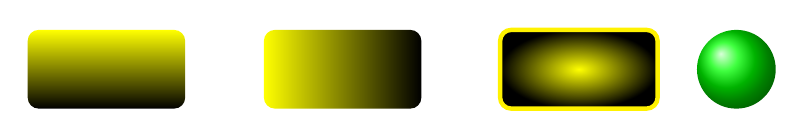
\begin{tikzpicture}[rounded corners, ultra thick]
		% (3, 0) rectangle +(2, 1) ==means==> 
		% (3, 0) rectangle (3 + 2, 0 + 1) ==> 
		% (3, 0) rectangle (5, 1)
		\shade[top color=yellow, bottom color=black] (0, 0) rectangle +(2, 1);
		\shade[left color=yellow, right color=black] (3, 0) rectangle +(2, 1);
		\shadedraw[inner color=yellow, outer color=black, draw=yellow] (6, 0) rectangle +(2, 1);
		\shade[ball color=green] (9, 0.5) circle (0.5cm);
	\end{tikzpicture}
\end{document}